\section{Grader} \label{sec:grader}
Når man regner på grafer, som vi vil gøre senere i projektet, kan det være brugbart at have styr på, hvor mange kanter der er incidente til en knude. Dertil bruger man følgende definition:

\begin{defn}[Grader] \label{defn:grader}
I en ikke orienteret graf er et punkts \emph{grader} det antal kanter, som punktet er incident med bortset fra løkker, som bidrager to gange til puntets grad. Punktet, v's, grader skrives $deg(v)$.
\end{defn}

Vi tager et eksempel:



\begin{figure}[H]
\centering
	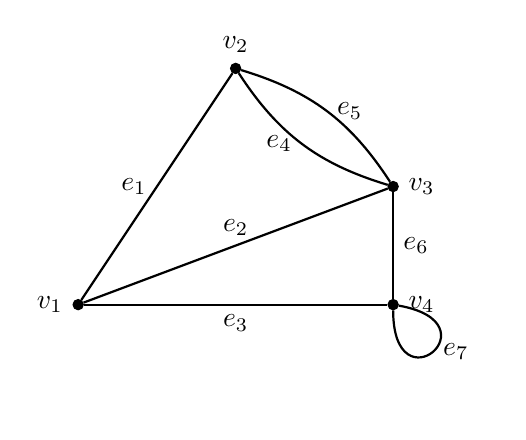
\begin{tikzpicture}[every loop/.style={}]
      \tikzset{enclosed/.style={draw, circle, inner sep=0pt, minimum size=.13cm, fill=black}}
%% Vertices
      	\node[enclosed, label={left: $v_1$}] (v1) at (0,0) {};
      	\node[enclosed, label={above: $v_2$}] (v2) at (2,3) {};
    	\node[enclosed, label={right: $v_3$}] (v3) at (4,1.5) {};
  	    \node[enclosed, label={right: $v_4$}] (v4) at (4,0) {};
%Edges
		\path[thick] (v2) edge [bend right=20] node[midway, left] {$e_4$} (v3);
		\path[thick] (v3) edge [bend right=20] node[midway, right] {$e_5$} (v2);
		\path[thick] (v1) edge node[midway, above] {$e_2$} (v3);
		\path[thick] (v1) edge node[midway, below] {$e_3$} (v4);
		\path[thick] (v1) edge node[midway, left] {$e_1$} (v2);
		\path[thick] (v3) edge node[midway, right] {$e_6$} (v4);
		\path[thick] (v4) edge [out=270,in=350,looseness=35] node[right] {$e_7$} (v4);
	\end{tikzpicture}
	\caption{Pseudograf.}
	\label{fig:grader}
\end{figure}


På figuren ses de forskellige punkter i en pseudograf og de kanter, der er incidente med hvert punkt. Graderne for de forskellige punkter ville her være: $deg(v_{1})=3, deg(v_{2})=3, deg(v_{3})=4$ og $deg(v_{4})=4$. Et punkts grader afgøres altså af hvor mange naboer punktet har, ved mindre punktet har en løkke, da man her kun siger, at den er nabo med sig selv én gang, men det tæller dobbelt i antallet af grader.